\documentclass{report}
\usepackage{graphicx, tikz-cd, float, titlepic, booktabs} % Required for inserting images
\usepackage{pgfplots}
\pgfplotsset{compat=1.15}
\usepackage{mathrsfs}
\usetikzlibrary{arrows}
\usepackage{amsmath, amssymb, amsthm, amsfonts, siunitx, physics, gensymb}
\AtBeginDocument{\RenewCommandCopy\qty\SI}
\usepackage[version=4]{mhchem}
\usepackage[most,many,breakable]{tcolorbox}
\usepackage{xcolor, fancyhdr, varwidth}
\usepackage[Glenn]{fncychap}
%Options: Sonny, Lenny, Glenn, Conny, Rejne, Bjarne, Bjornstrup
\usepackage{hyperref, cleveref}
\usepackage{icomma, enumitem} %comma as decimal and continue enumerate with [resume]
\usepackage[danish]{babel}
%%%%%%%%%%%%%%%%%%%%%%%%%%%%%%
% SELF MADE COLORS
%%%%%%%%%%%%%%%%%%%%%%%%%%%%%%
\definecolor{myg}{RGB}{56, 140, 70}
\definecolor{myb}{RGB}{45, 111, 177}
\definecolor{myr}{RGB}{199, 68, 64}
\definecolor{mytheorembg}{HTML}{F2F2F9}
\definecolor{mytheoremfr}{HTML}{00007B}
\definecolor{mylenmabg}{HTML}{FFFAF8}
\definecolor{mylenmafr}{HTML}{983b0f}
\definecolor{mypropbg}{HTML}{f2fbfc}
\definecolor{mypropfr}{HTML}{191971}
\definecolor{myexamplebg}{HTML}{F2FBF8}
\definecolor{myexamplefr}{HTML}{88D6D1}
\definecolor{myexampleti}{HTML}{2A7F7F}
\definecolor{mydefinitbg}{HTML}{E5E5FF}
\definecolor{mydefinitfr}{HTML}{3F3FA3}
\definecolor{notesgreen}{RGB}{0,162,0}
\definecolor{myp}{RGB}{197, 92, 212}
\definecolor{mygr}{HTML}{2C3338}
\definecolor{myred}{RGB}{127,0,0}
\definecolor{myyellow}{RGB}{169,121,69}
\definecolor{myexercisebg}{HTML}{F2FBF8}
\definecolor{myexercisefg}{HTML}{88D6D1}
%%%%%%%%%%%%%%%%%%%%%%%%%%%%%%%%%%%%%%%%%%%%%%%%%%%%%%%%%%%%%%%%%%%%%%
% Box environments for theorems and problems
%%%%%%%%%%%%%%%%%%%%%%%%%%%%%%%%%%%%%%%%%%%%%%%%%%%%%%%%%%%%%%%%%%%%%
\setlength{\parindent}{1cm}
%================================
% Question BOX
%================================
\makeatletter
\newtcbtheorem{question}{Opgave}{enhanced,
	breakable,
	colback=white,
	colframe=myb!80!black,
	attach boxed title to top left={yshift*=-\tcboxedtitleheight},
	fonttitle=\bfseries,
	title={#2},
	boxed title size=title,
	boxed title style={%
			sharp corners,
			rounded corners=northwest,
			colback=tcbcolframe,
			boxrule=0pt,
		},
	underlay boxed title={%
			\path[fill=tcbcolframe] (title.south west)--(title.south east)
			to[out=0, in=180] ([xshift=5mm]title.east)--
			(title.center-|frame.east)
			[rounded corners=\kvtcb@arc] |-
			(frame.north) -| cycle;
		},
	#1
}{def}
\makeatother
%================================
% DEFINITION BOX
%================================

\newtcbtheorem[]{Definition}{Definition}{enhanced,
	before skip=2mm,after skip=2mm, colback=red!5,colframe=red!80!black,boxrule=0.5mm,
	attach boxed title to top left={xshift=1cm,yshift*=1mm-\tcboxedtitleheight}, varwidth boxed title*=-3cm,
	boxed title style={frame code={
					\path[fill=tcbcolback]
					([yshift=-1mm,xshift=-1mm]frame.north west)
					arc[start angle=0,end angle=180,radius=1mm]
					([yshift=-1mm,xshift=1mm]frame.north east)
					arc[start angle=180,end angle=0,radius=1mm];
					\path[left color=tcbcolback!60!black,right color=tcbcolback!60!black,
						middle color=tcbcolback!80!black]
					([xshift=-2mm]frame.north west) -- ([xshift=2mm]frame.north east)
					[rounded corners=1mm]-- ([xshift=1mm,yshift=-1mm]frame.north east)
					-- (frame.south east) -- (frame.south west)
					-- ([xshift=-1mm,yshift=-1mm]frame.north west)
					[sharp corners]-- cycle;
				},interior engine=empty,
		},
	fonttitle=\bfseries,
	title={#2},#1}{def}
\newtcbtheorem[]{definition}{Definition}{enhanced,
	before skip=2mm,after skip=2mm, colback=red!5,colframe=red!80!black,boxrule=0.5mm,
	attach boxed title to top left={xshift=1cm,yshift*=1mm-\tcboxedtitleheight}, varwidth boxed title*=-3cm,
	boxed title style={frame code={
					\path[fill=tcbcolback]
					([yshift=-1mm,xshift=-1mm]frame.north west)
					arc[start angle=0,end angle=180,radius=1mm]
					([yshift=-1mm,xshift=1mm]frame.north east)
					arc[start angle=180,end angle=0,radius=1mm];
					\path[left color=tcbcolback!60!black,right color=tcbcolback!60!black,
						middle color=tcbcolback!80!black]
					([xshift=-2mm]frame.north west) -- ([xshift=2mm]frame.north east)
					[rounded corners=1mm]-- ([xshift=1mm,yshift=-1mm]frame.north east)
					-- (frame.south east) -- (frame.south west)
					-- ([xshift=-1mm,yshift=-1mm]frame.north west)
					[sharp corners]-- cycle;
				},interior engine=empty,
		},
	fonttitle=\bfseries,
	title={#2},#1}{def}

\newtcbtheorem{theo}%
    {Theorem}{}{theorem}
\newtcolorbox{prob}[1]{colback=red!5!white,colframe=red!50!black,fonttitle=\bfseries,title={#1}}
%================================
% NOTE BOX
%================================

\usetikzlibrary{arrows,calc,shadows.blur}
\tcbuselibrary{skins}
\newtcolorbox{note}[1][]{%
	enhanced jigsaw,
	colback=gray!20!white,%
	colframe=gray!80!black,
	size=small,
	boxrule=1pt,
	title=\textbf{Note:},
	halign title=flush center,
	coltitle=black,
	breakable,
	drop shadow=black!50!white,
	attach boxed title to top left={xshift=1cm,yshift=-\tcboxedtitleheight/2,yshifttext=-\tcboxedtitleheight/2},
	minipage boxed title=1.5cm,
	boxed title style={%
			colback=white,
			size=fbox,
			boxrule=1pt,
			boxsep=2pt,
			underlay={%
					\coordinate (dotA) at ($(interior.west) + (-0.5pt,0)$);
					\coordinate (dotB) at ($(interior.east) + (0.5pt,0)$);
					\begin{scope}
						\clip (interior.north west) rectangle ([xshift=3ex]interior.east);
						\filldraw [white, blur shadow={shadow opacity=60, shadow yshift=-.75ex}, rounded corners=2pt] (interior.north west) rectangle (interior.south east);
					\end{scope}
					\begin{scope}[gray!80!black]
						\fill (dotA) circle (2pt);
						\fill (dotB) circle (2pt);
					\end{scope}
				},
		},
	#1,
}
%================================
% EXAMPLE BOX
%================================
\newtcbtheorem[number within=section]{Example}{Example}
{%
	colback = myexamplebg
	,breakable
	,colframe = myexamplefr
	,coltitle = myexampleti
	,boxrule = 1pt
	,sharp corners
	,detach title
	,before upper=\tcbtitle\par\smallskip
	,fonttitle = \bfseries
	,description font = \mdseries
	,separator sign none
	,description delimiters parenthesis
}
{ex}
%================================
% THEOREM BOX
%================================

\tcbuselibrary{theorems,skins,hooks}
\newtcbtheorem[number within=section]{Theorem}{Theorem}
{%
	enhanced,
	breakable,
	colback = mytheorembg,
	frame hidden,
	boxrule = 0sp,
	borderline west = {2pt}{0pt}{mytheoremfr},
	sharp corners,
	detach title,
	before upper = \tcbtitle\par\smallskip,
	coltitle = mytheoremfr,
	fonttitle = \bfseries\sffamily,
	description font = \mdseries,
	separator sign none,
	segmentation style={solid, mytheoremfr},
}
{th}
%%%%%%%%%%%%%%%%%%%%%%%%%%%%%%%%%%%%%%%%%%%%%%%%%%%%%%%%%%%%%%%%%
% SELF MADE COMMANDS
%%%%%%%%%%%%%%%%%%%%%%%%%%%%%%
\newcommand{\sol}{\setlength{\parindent}{0cm}\textbf{\textit{Løsning:}}\setlength{\parindent}{1cm}}
%%%%%%%%%%%%%%%%%%%%%%%%%%%%%%%%%
\usepackage[tmargin=2cm,rmargin=1in,lmargin=1in,margin=0.85in,bmargin=2cm,footskip=.2in]{geometry}\pagestyle{fancy}
\lhead{Minrui Kevin Zhou 2.b}
\rhead{Indgreb i ligevægt}

\title{Rapport 3: Indgreb i ligevægt\\
{\Large \textbf{2.b kemi A}}}
\author{Kevin Zhou}
\date{\today}
\titlepic{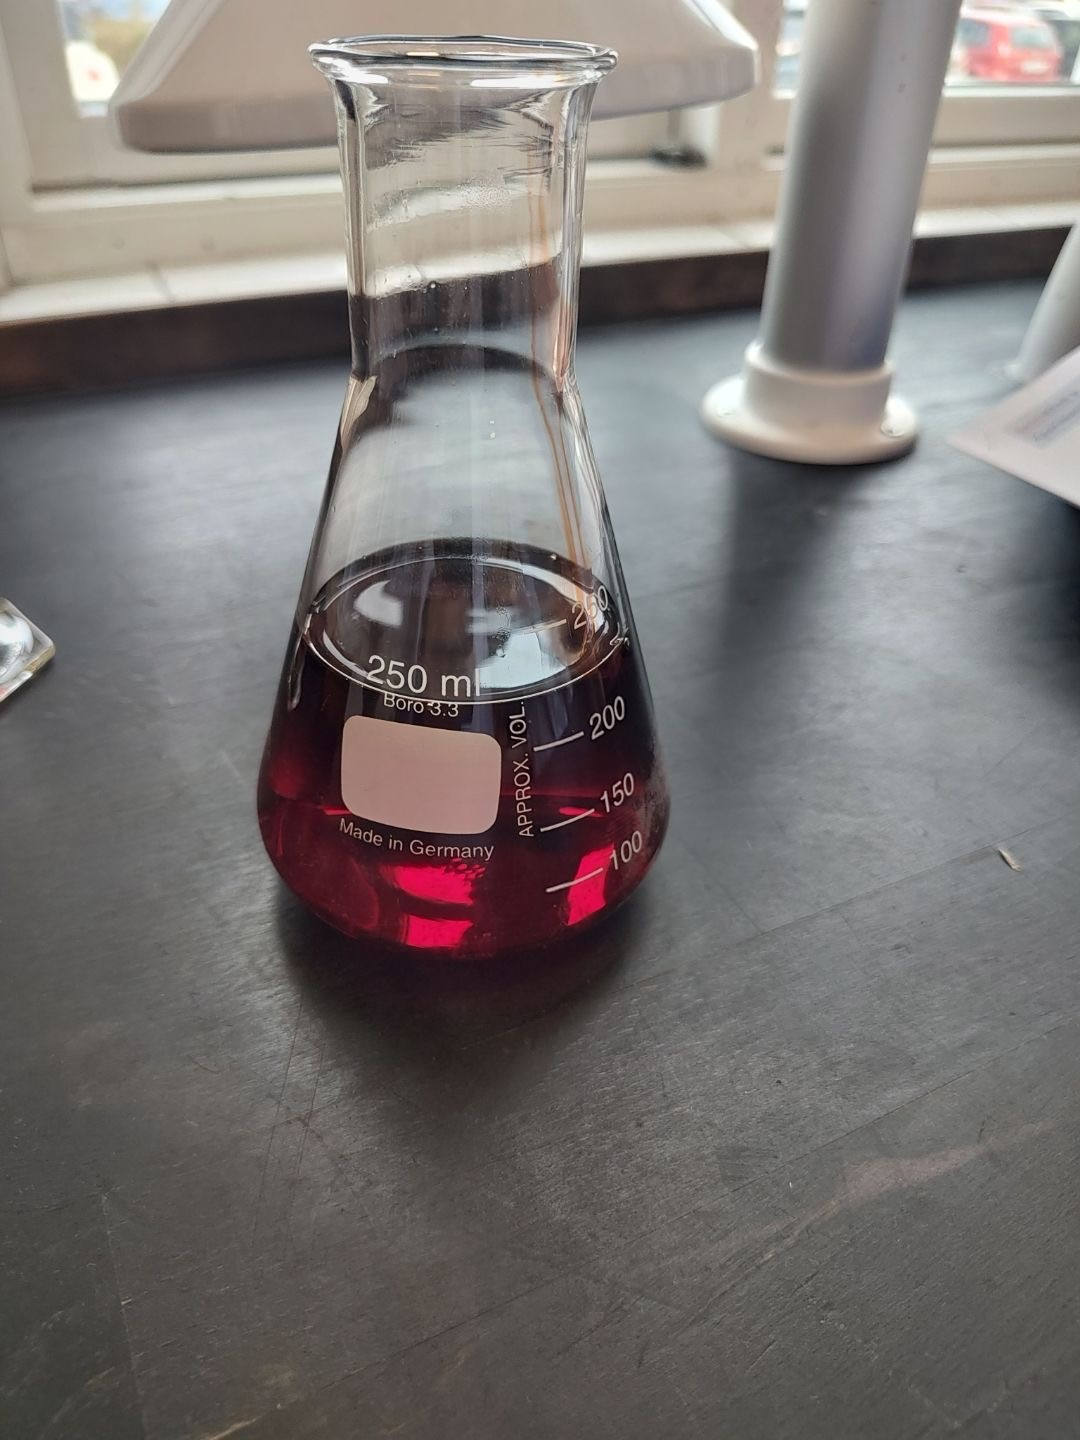
\includegraphics[width=0.7\textwidth]{konisk.jpeg}}
\begin{document}
\maketitle
\section*{Formål}
Formålet med eksperimentet er at undersøge forskydningen af en kemisk ligevægt ved forskellige indgreb, især med hensyn til Le Chateliers princip.
Ligevægten vi undersøger er hvor jern(3+)ioner reagerer med thiocyanat (\ce{SCN-}) og danner en kompleks ion. 
Reaktionsskemaet for ligevægten ses i Teori.
\section*{Teori}
I reaktionsskema \ref{rea:ligevægt} ses reaktionsskemaet for den undersøgte ligevægt, hvor den komplekse ion til højre er rød.
\begin{equation}
\label{rea:ligevægt}
\begin{split}
  \ce{Fe^3+(aq) + SCN-(aq) <=> $\underset{\text{rød}}{\ce{FeSCN^2+(aq)}}$} 
\end{split}
\end{equation}
Siden ionen til højre er rød, så er det da klart, at opløsningens farve bliver mere rød ved en forskydning mod højre.
Omvendt bliver opløsningens farve mindre rød og mere farveløs ved en forskydning mod venstre.
Ligevægtsloven for ligevægten ses i ligning \ref{eq:ligevægt}.
\begin{equation}
  \label{eq:ligevægt}
\begin{split}
  \frac{[\ce{FeSCN^2+}]}{[\ce{Fe^3+}]\cdot [\ce{SCN-}]}=K_c
\end{split}
\end{equation}

Vi vil i teorien her også kort introducere Le Chaterliers princip.
\begin{Theorem*}{Le Chateliers princip}{}
Et ydre indgreb i et ligevægtssystem fremkalder en forskydning, som formindsker virkningen af indgrebet.
\end{Theorem*}
Dette princip kan vi så bruge til at forudsige og begrunde forskydningernes retninger i forsøgene.
Vi spørger da os selv om, hvilken retning forskydningen skal ske for at det ydre indgreb mindskes.

Det er også relevant for delforsøg 2 at vide, at ascorbinsyre reducerer \ce{Fe^3+} til \ce{Fe^2+}.
\section*{Apparatur, kemikalier og sikkerhed}

\subsection*{Apparatur}
\begin{itemize}
  \item 7 reagensglas i stativ
  \item Konisk kolbe, $250 \;\unit{mL} $
\item 2 måleglas, $10 \;\unit{mL} $
\item Termometer
\item Spatler
\item 2 bægerglas, $250 \;\unit{mL} $
\item 2 ens bægerglas, $100 \;\unit{mL} $
\end{itemize}
\subsection*{Kemikalier}
\begin{itemize}
  \item $0,1 \;\unit{\textsc{m}}$ jern(3+)nitrat, \ce{Fe(NO3)3} 
\item $0,1 \;\unit{\textsc{m}}$ kaliumthiocyanat, KSCN 
\item Farvet vand
  \item $0,1 \;\unit{\textsc{m}}$ sølv(1+)nitrat, \ce{AgNO3} 
  \item Jern(3+)nitrat, \ce{Fe(NO3)3} 
\item Ascorbinsyre
\item Kaliumthiocyanat, KSCN
\item Isterninger
\end{itemize}
\subsection*{Sikkerhed}
\begin{itemize}
  \item $0,1 \;\unit{\sc{m}}$ sølv(1+)nitrat er ætsende og giver sorte pletter på tøj og hud.
\item Kaliumthiocyanat er farlig ved indånding og kan udvikle giftig gas ved kontakt med syre.
  \item Jern(3+)nitrat kan irritere hud og øjne.
\end{itemize}

\section*{Udførelse}
Først fyldes cirka $200 \;\unit{mL} $ vand i en $250 \;\unit{mL} $ konisk kolbe.
Der tilsættes herefter $10 \;\unit{mL} $ $0,1 \;\unit{\textsc{m}} $ \ce{KSCN}.
Opløsningen blandes med en spatel og iagttagelserne noteres ned.
En del af opløsningen overføres til syv reagensglas, der fyldes en tredjedel op, og bruges til seks forskellige delforsøg.
Disse reagensglas med opløsningen betegnes herefter som reagensglas 1-7.
\subsection*{Delforsøg 1}
En spatelfuld fast \ce{Fe(NO3)3} overføres til reagensglas 1, hvorefter der røres rundt.
Iagttagelserne noteres ned.
\subsection*{Delforsøg 2a}
Nogle få \unit{mL} $0,1 \textsc{m}$ \ce{Fe(NO3)3}-opløsning hældes op i et reagensglas og spatelspidser af ascorbinsyre tilsættes indtil en ændring ses.
\subsection*{Delforsøg 2b}
En spatelspids ascorbinsyre tilsættes til reagensglas 2, hvorefter der røres rundt.
Iagttageleserne noteres ned.
\subsection*{Delforsøg 3}
Der tilsættes en spatelspids \ce{KSCN} til reagensglas 3, hvorefter der røres rundt.
Iagttageleserne noteres ned.
\subsection*{Delforsøg 4a}
Nogle få \unit{mL} $0,1 \;\unit{\textsc{m}} $ \ce{KSCN}-opløsning hældes op i et reagensglas, hvorefter et par dråber $0,1 \;\unit{\textsc{m}} $ \ce{AgNO3} tilsættes.
Iagttageleserne noteres ned.
\subsection*{Delforsøg 4b}
Til reagensglas 4 tilsættes et par dråber $0,1 \;\unit{\textsc{m}} $ \ce{AgNO3}, hvorefter der røres rundt.
Iagttageleserne noteres ned.
\subsection*{Delforsøg 5+6}
Der laves et vandbad med $50 \;\unit{\celsius} $ vand i et $250 \;\unit{mL} $ bægerglas samt et isband i et andet bægerglas.
Reagensglas 5 placeres så i det varme bad og reagensglas 6 i isbaddet.
Efter et stykke tid sammenlignes de med reagensglas 7.
\subsection*{Delforsøg 7a}
Der stilles to $100 \;\unit{mL} $ bægerglas ved siden af hinanden på et hvidt papir og fyldes næsten halvt op med farvet vand sådan, at væsken står nøjagtigt lige højt i de to glas.
Volumenet i det ene bægerglas fordobles da ved tilsætning af vand.
Farveintensiteten af de to bægerglas sammenlignes.
\subsection*{Delforsøg 7b}
Et tilsvarende forsøg som i 7a laves, hvor der i stedet for farvet vand bruges den røde ligevægtsblanding fra den koniske kolbe.
\section*{Resultater}
Ved blandingen af opløsningen i den koniske kolbe, bliver den rød, hvilket ses i \cref{fig:kolbe}.
Reaktionshastigheden er stor.
\begin{figure}[H]
\begin{center}
  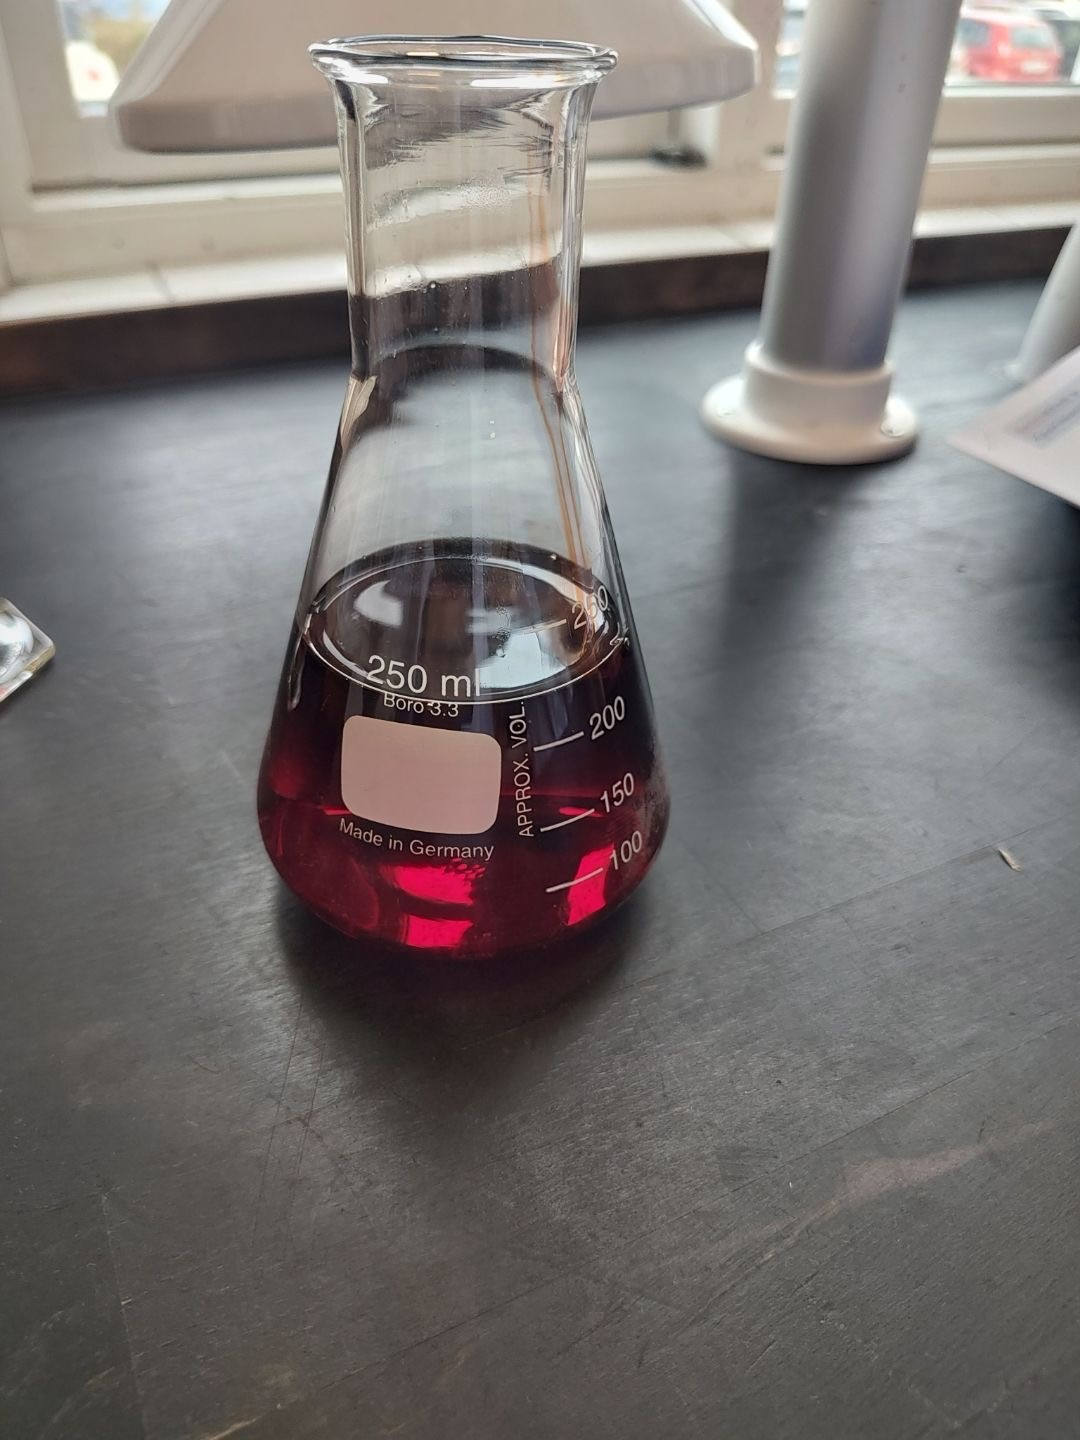
\includegraphics[scale=0.4]{konisk.jpeg}
\end{center}
\caption{Opløsningen i kolben er rød, når ligevægten har indstillet sig}
\label{fig:kolbe}
\end{figure}
\subsection*{Delforsøg 1}
Ved tilsætningen af \ce{Fe(NO3)3} bliver opløsningen i reagensglas 1 lidt rødere, hvilket ses i \cref{fig:for1}.
Bemærk, at det er svært at se, at opløsningen er blevet rødere, da vi glemte at sammenligne med reagensglas 7.
\begin{figure}[H]
\begin{center}
  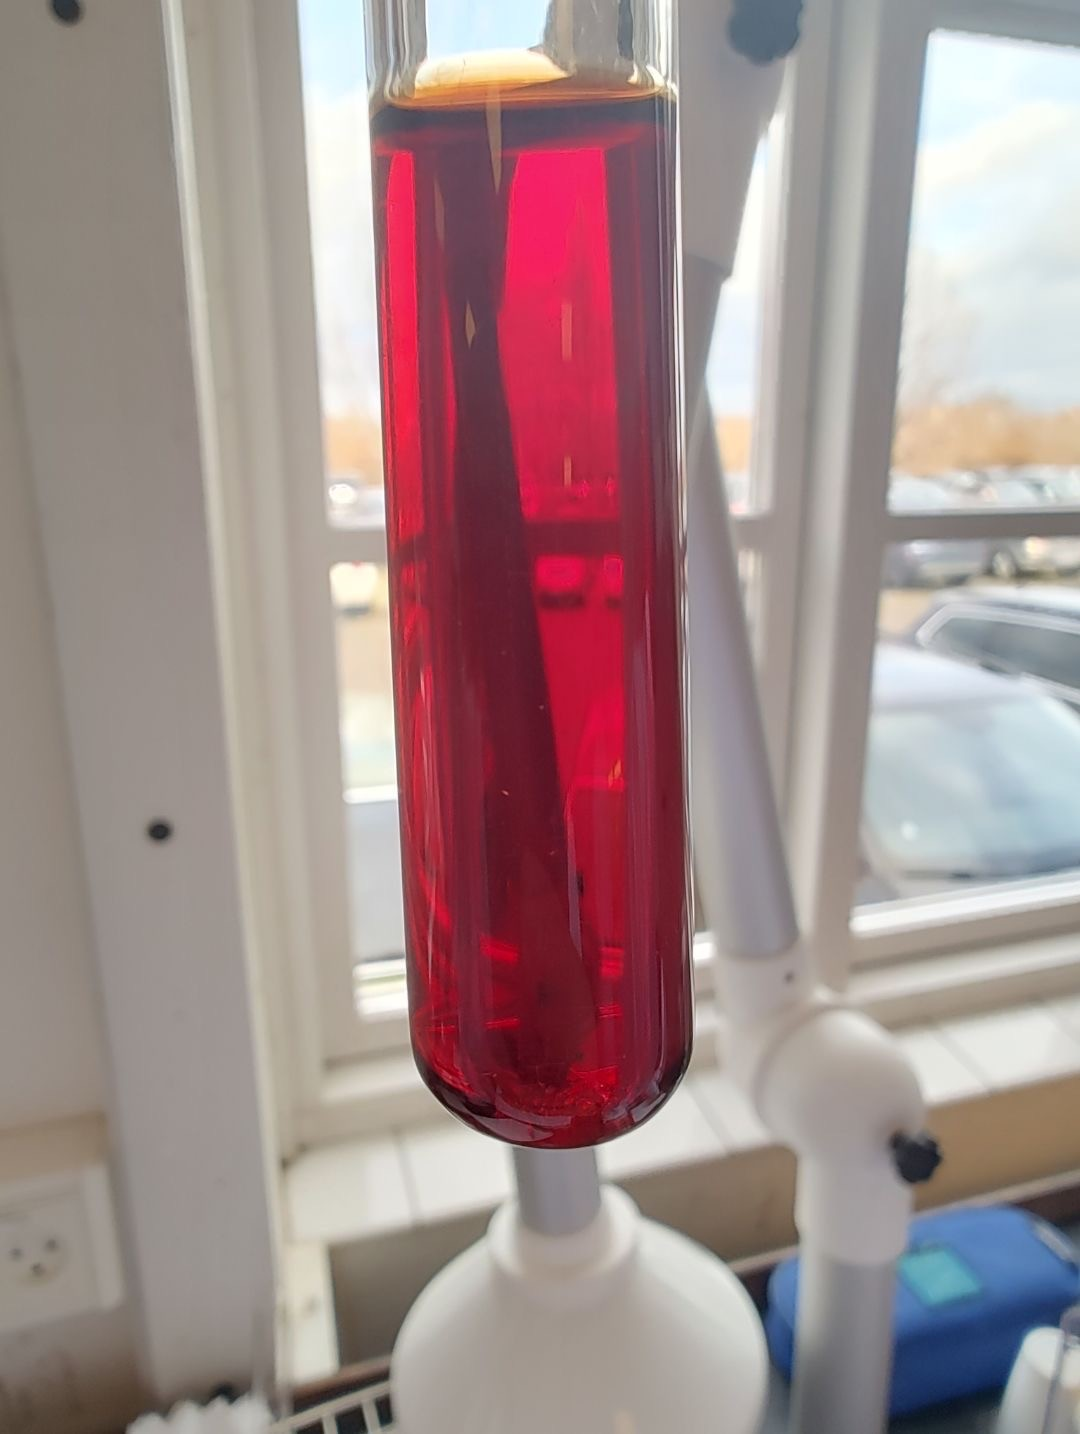
\includegraphics[scale=0.25]{for1.jpeg}
\end{center}
  \caption{Reagensglas 1 efter tilsætning af \ce{Fe(NO3)3}}
\label{fig:for1}
\end{figure}

\subsection*{Delforsøg 2a + 2b}
I delforsøg 2a går opløsningens farve fra gul til farveløs.
I delforsøg 2b går opløsningens farve fra rød til farveløs, hvilket ses i \cref{fig:for2}.
\begin{figure}[H]
\begin{center}
  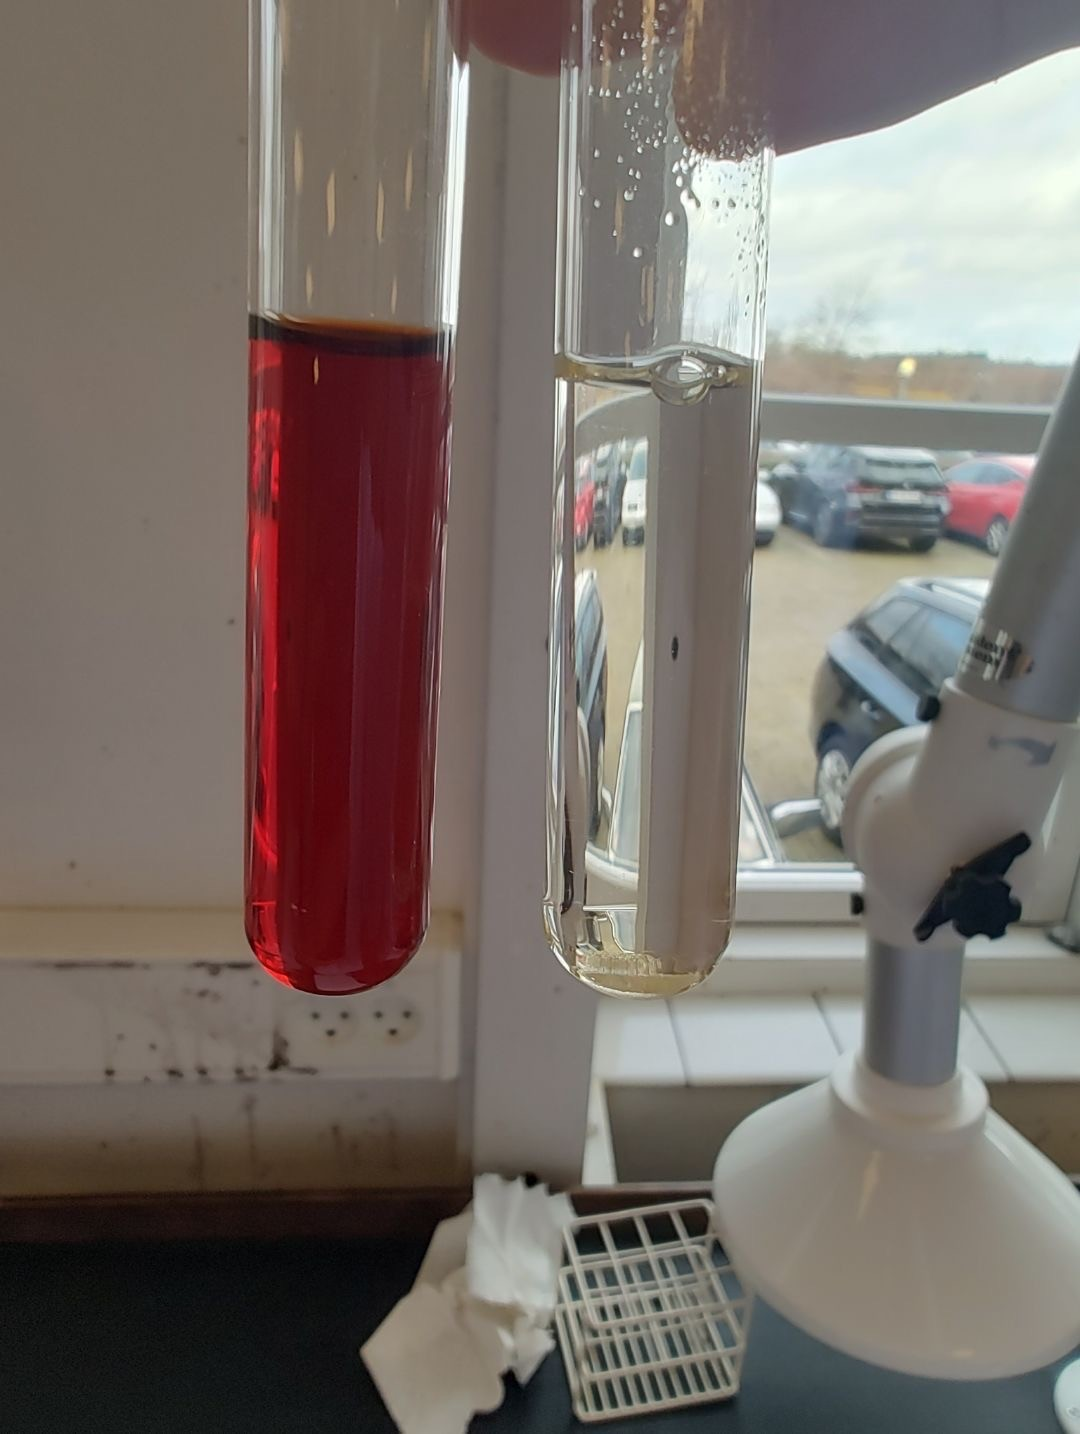
\includegraphics[scale=0.23]{for2.jpeg}
\end{center}
\caption{Reagensglas 2 efter tilsætning af ascorbinsyre med reagensglas 7 til sammenligning}
\label{fig:for2}
\end{figure}
\subsection*{Delforsøg 3}
Ved tilsætningen af \ce{KSCN} går opløsningens farve i reagensglas 3 fra rød til mørkerød, hvilket ses i \cref{fig:for3}, hvor reagensglas 7 er med for sammenligning.
\begin{figure}[H]
\begin{center}
  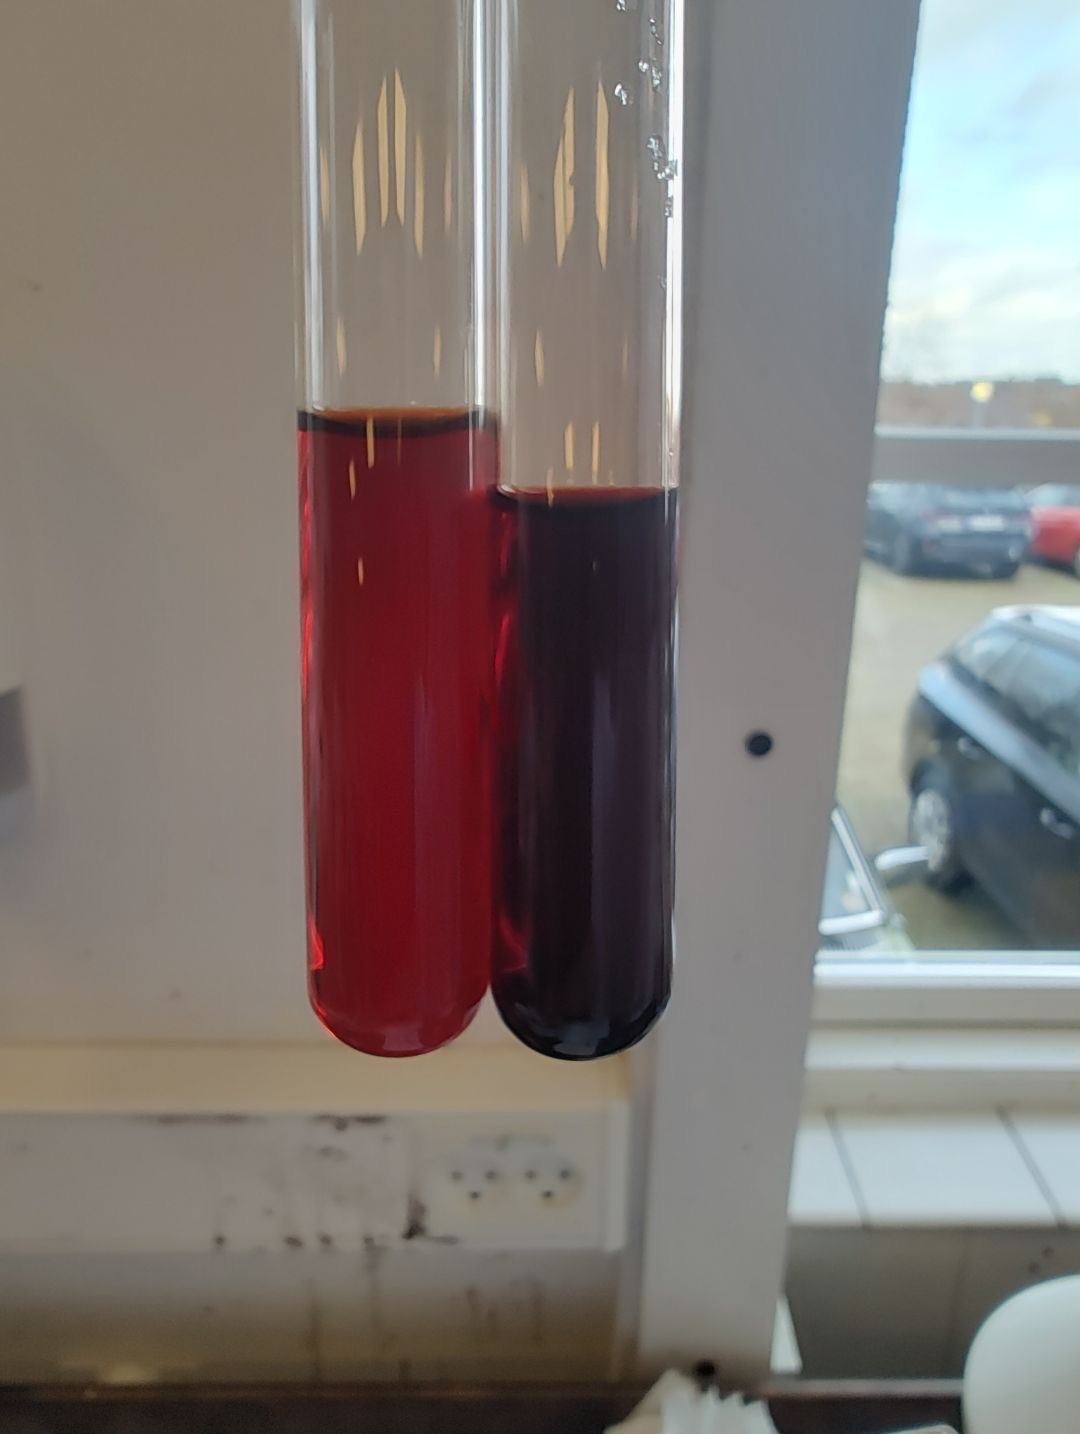
\includegraphics[scale=0.2]{for3.jpeg}
\end{center}
\caption{Reagensglas 3 efter tilsætning af \ce{KSCN}}
\label{fig:for3}
\end{figure}
\subsection*{Delforsøg 4a}
Ved tilsætning af \ce{AgNO3}-opløsning til \ce{KSCN}-opløsningen dannes der hvidt bundfald, hvilket ses i \cref{fig:for4a}.
\begin{figure}[H]
\begin{center}
  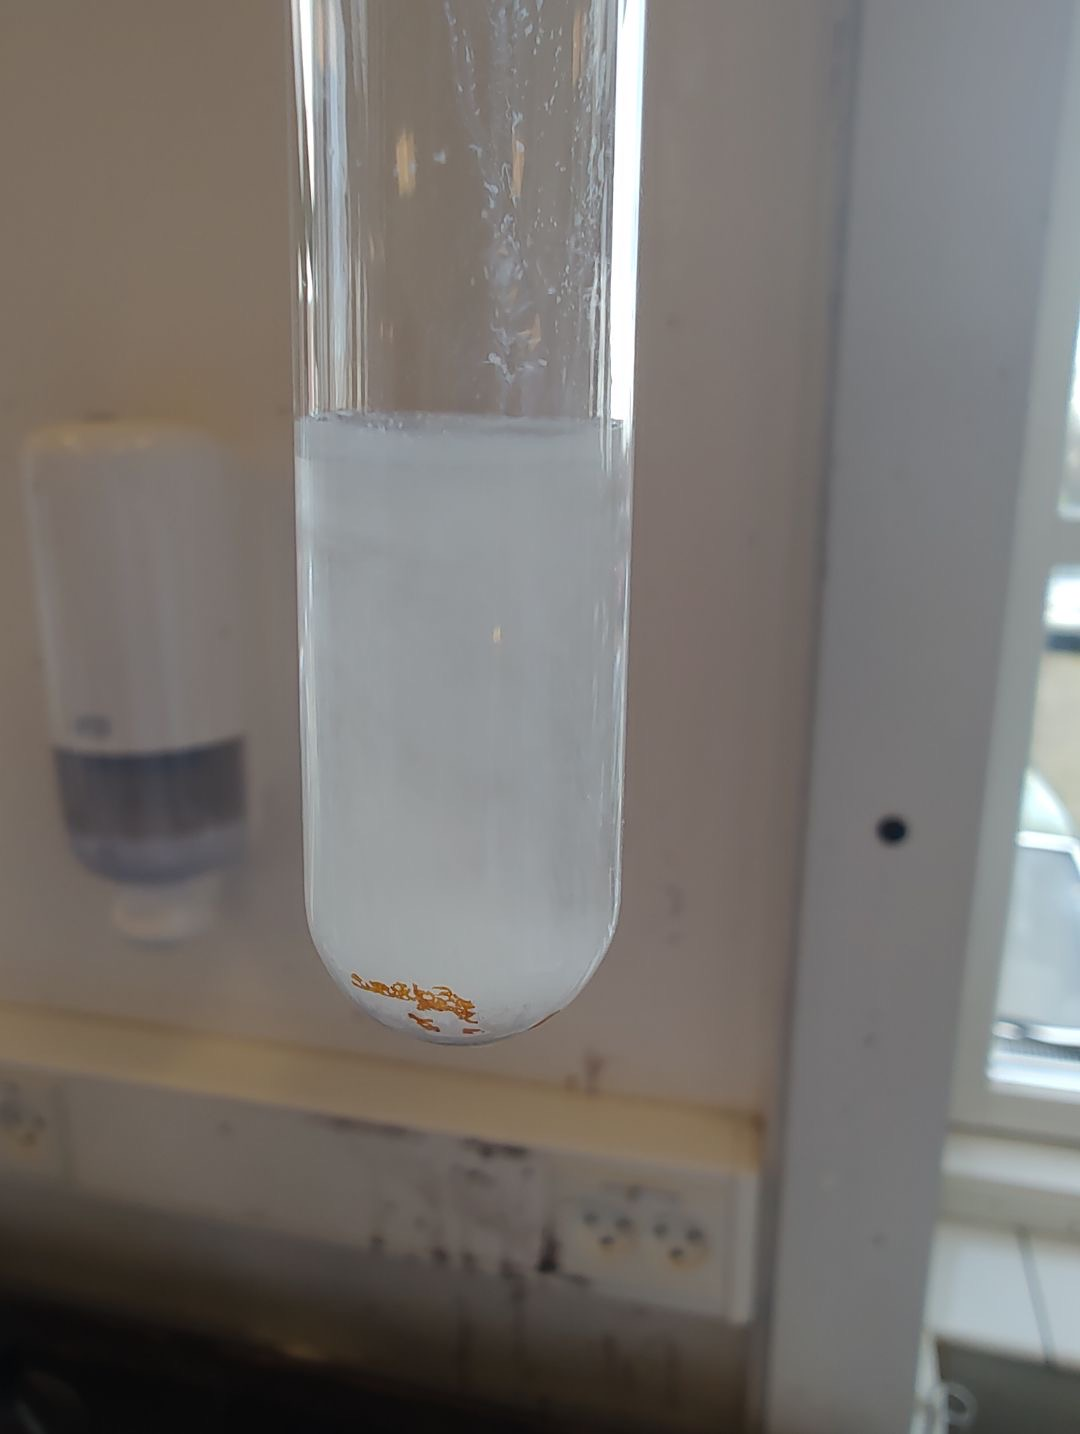
\includegraphics[scale=0.18]{for4a.jpeg}
\end{center}
\caption{Hvidt bundfald dannes ved tilsætningen af \ce{AgNO3}-opløsning til \ce{KSCN}-opløsningen}
\label{fig:for4a}
\end{figure}
\subsection*{Delforsøg 4b}
Ved tilsætning af \ce{AgNO3}-opløsning til reagensglas 4 dannes der hvidt bundfald, hvilket ses i \cref{fig:for4b}.
\begin{figure}[H]
\begin{center}
  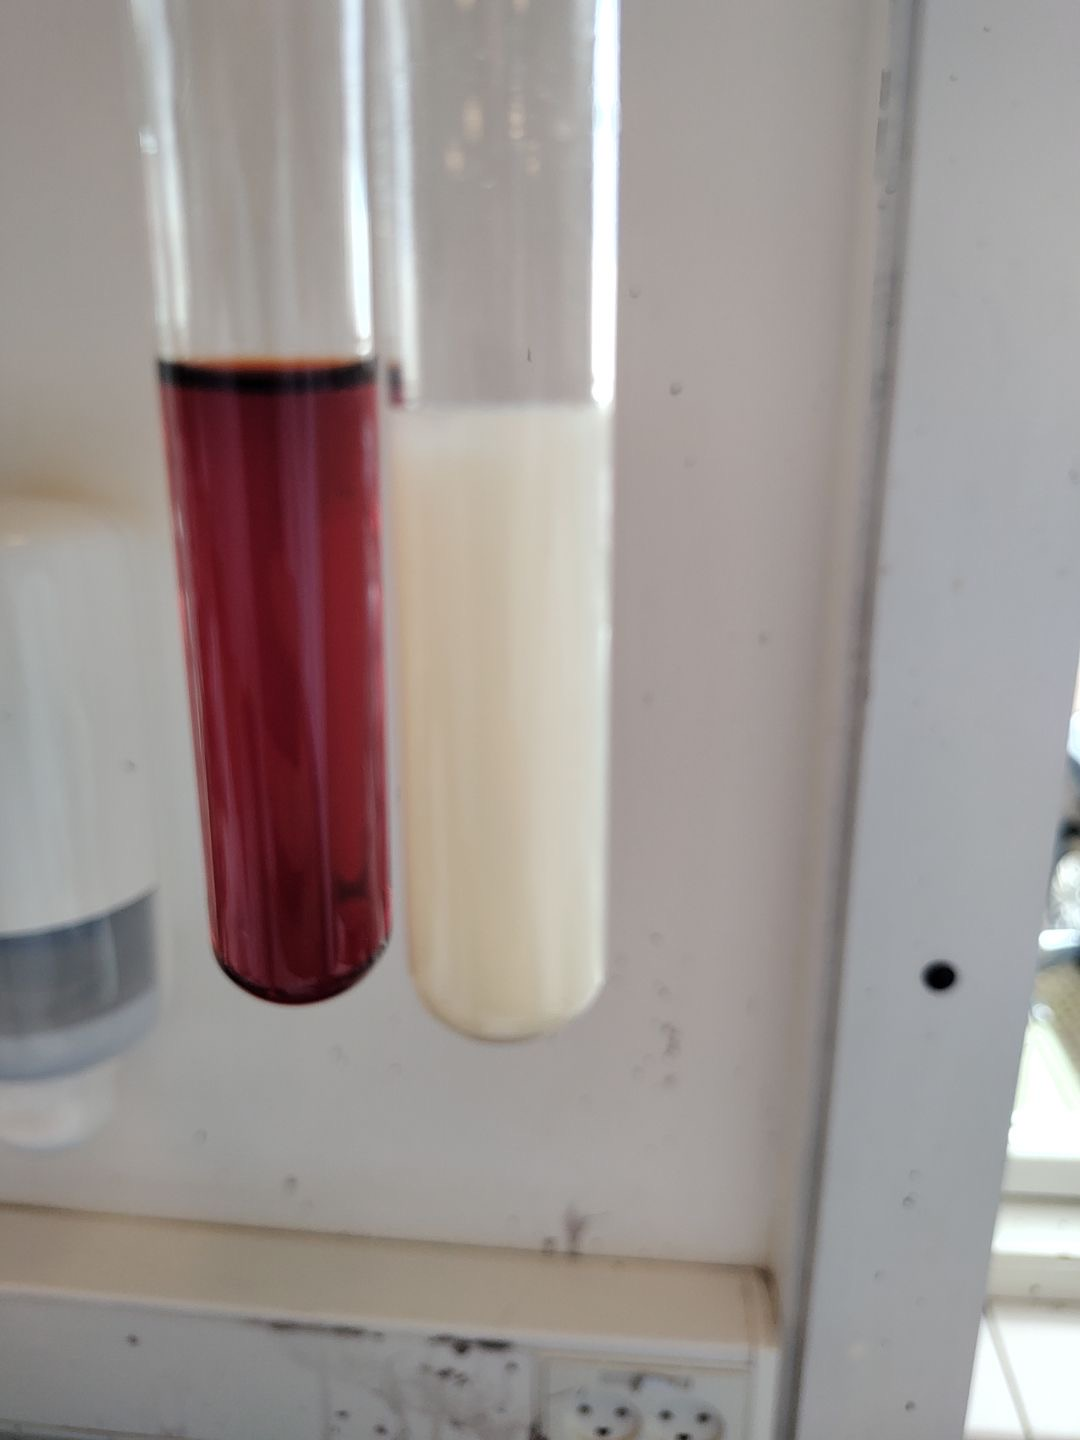
\includegraphics[scale=0.2]{for4b.jpeg}
\end{center}
\caption{Reagensglas 4 efter tilsætning af \ce{AgNO3}-opløsning}
\label{fig:for4b}
\end{figure}
\subsection*{Delforsøg 5+6}
Reagensglas 5 er blevet mindre rød ved opvarmning, hvor reagensglas 6 er blevet mere mørkerød ved afkøling.
De ses ved siden af hinanden i \cref{fig:for5}.
\begin{figure}[H]
\begin{center}
  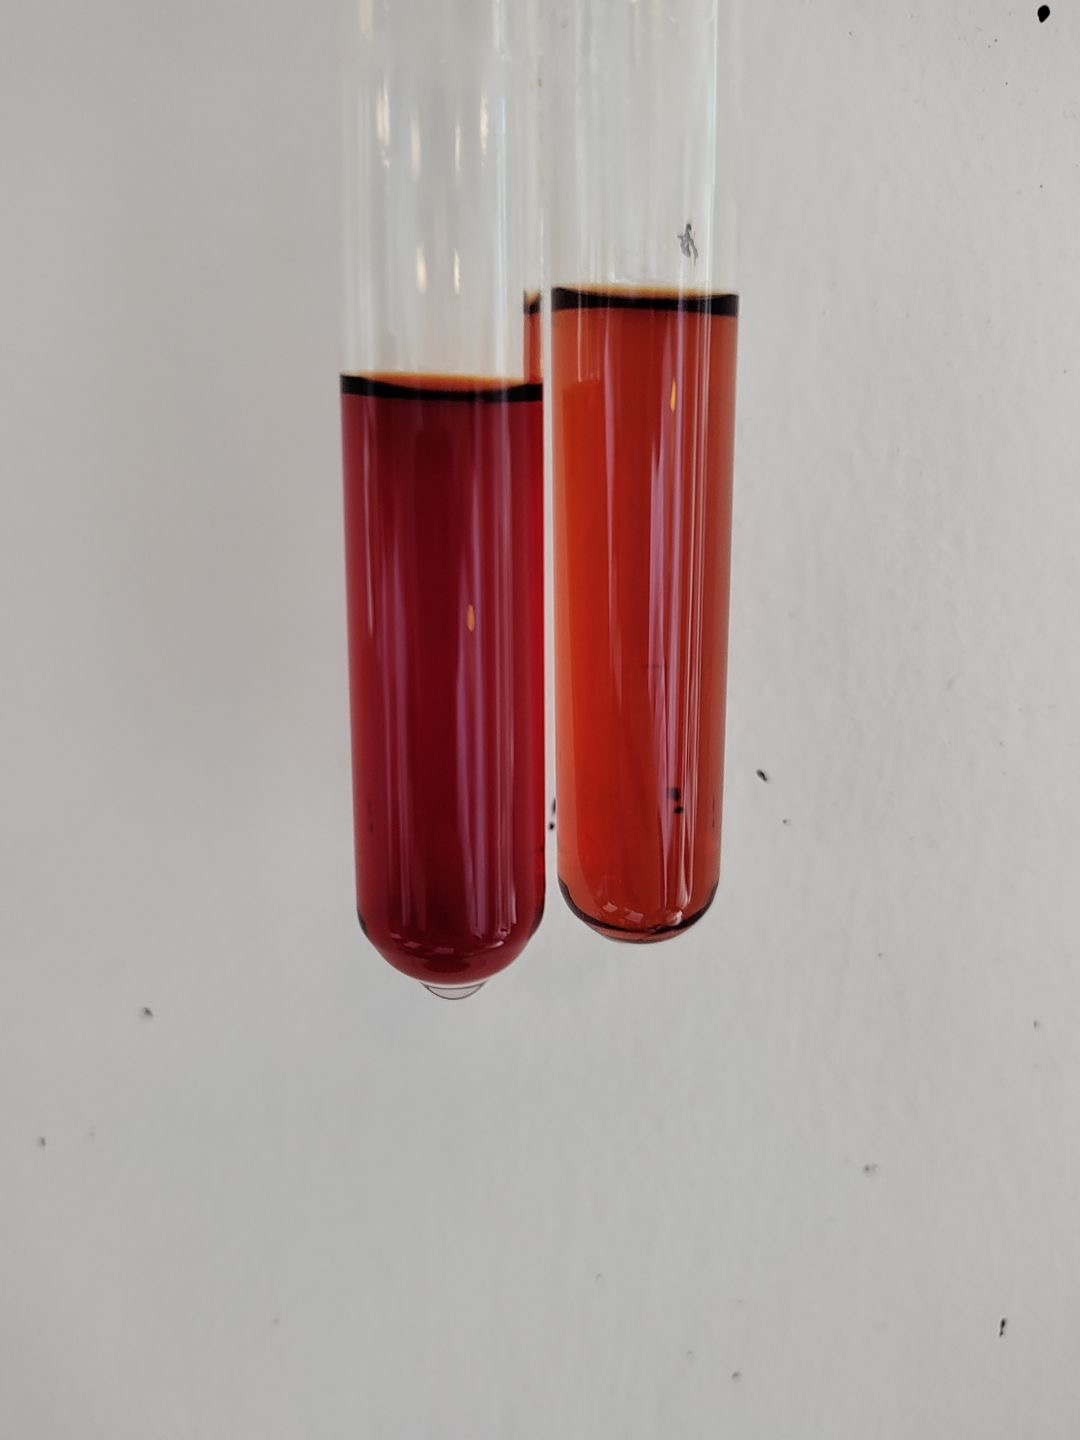
\includegraphics[scale=0.18]{for5.jpeg}
\end{center}
  \caption{Reagensglas 5 (th.) og 6 (tv.) ved siden af hinanden}
\label{fig:for5}
\end{figure}
\subsection*{Delforsøg 7a}
Vi ser da, at den fortyndede opløsnings farve er lysere set fra siden, men den samme set oppefra, hvilket ses i \cref{fig:7aa} og \cref{fig:7ab}.
\begin{figure}[H]
\begin{center}
  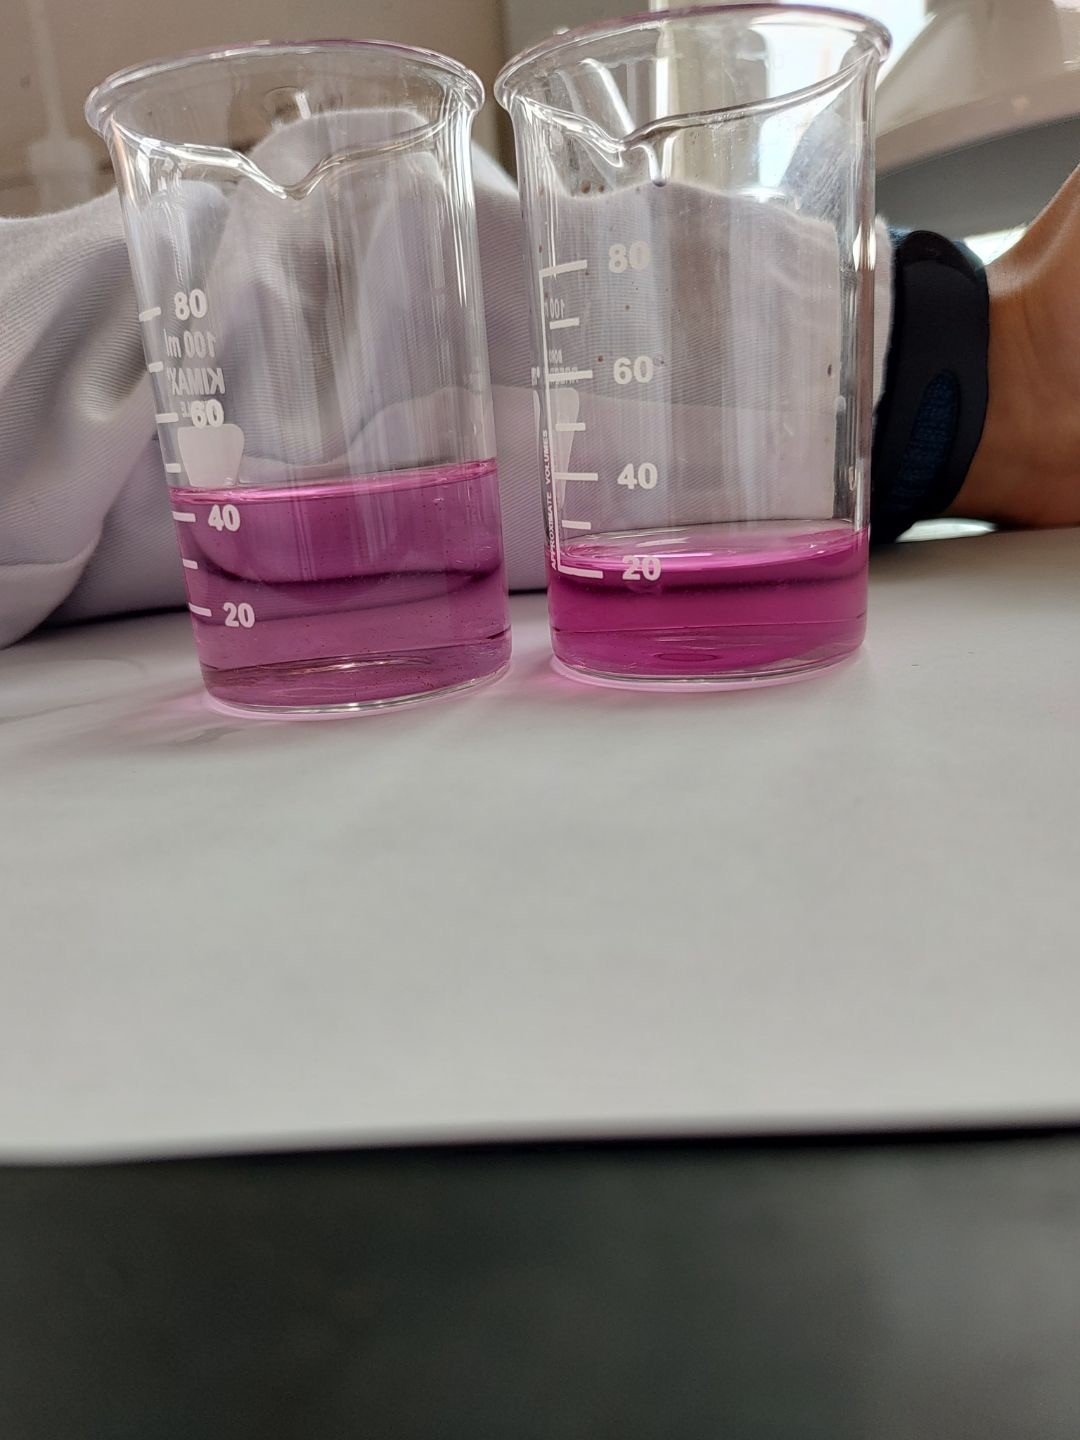
\includegraphics[scale=0.23]{for7aa.jpeg}
\end{center}
\caption{De to bægerglas set fra siden}
\label{fig:7aa}
\end{figure}
\begin{figure}[H]
\begin{center}
  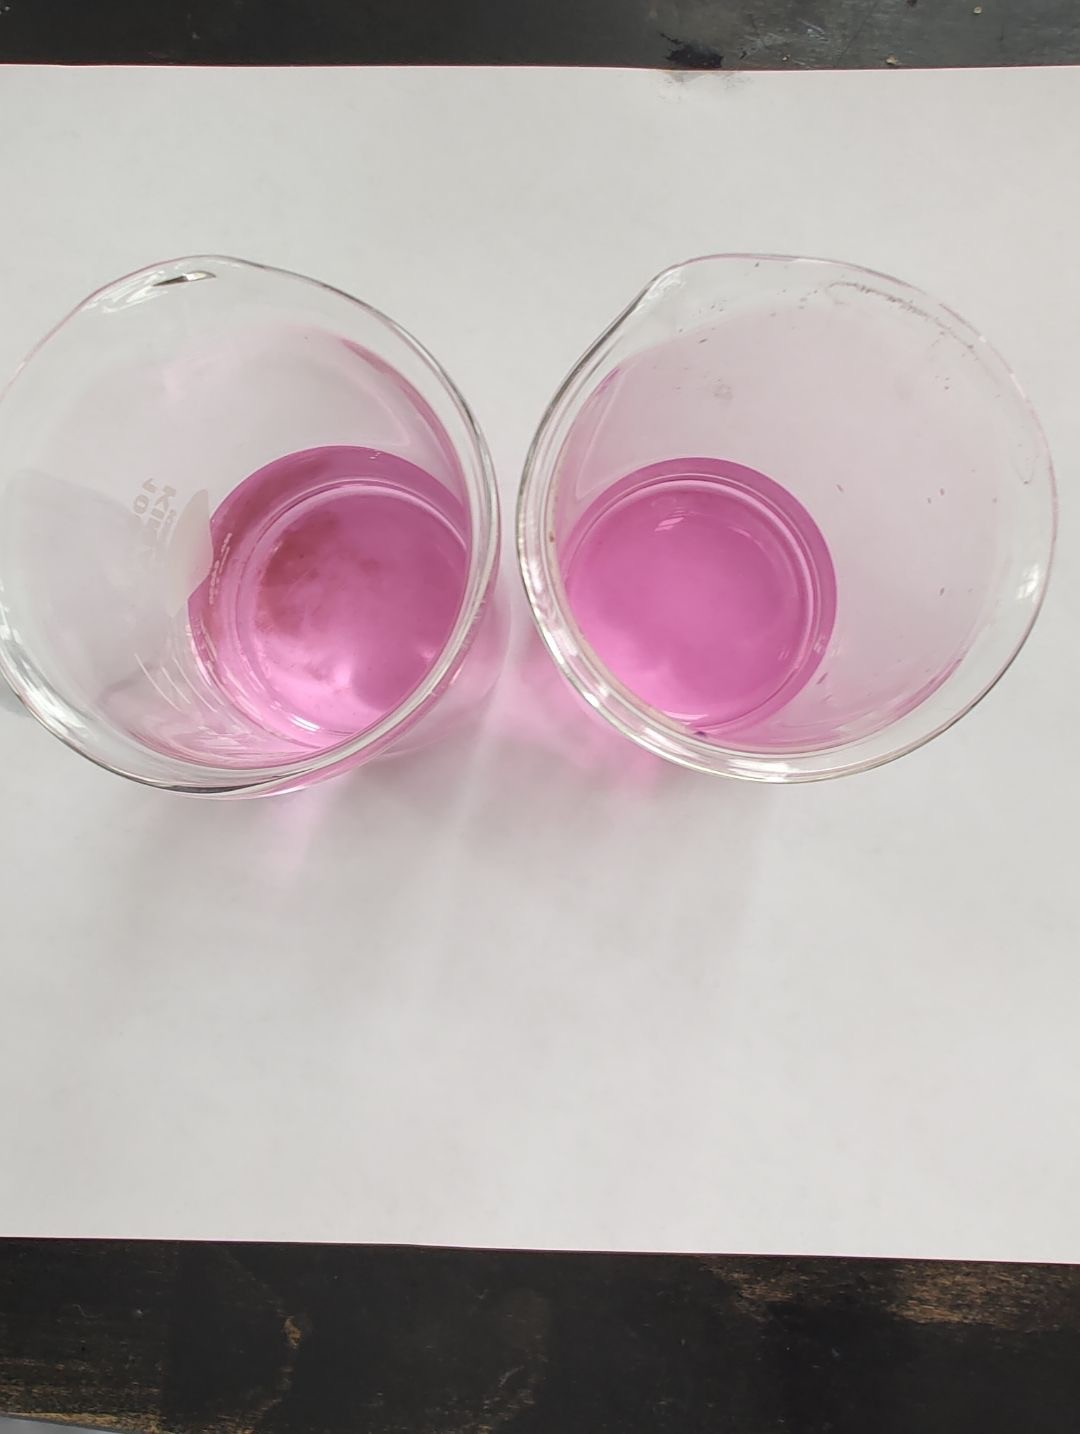
\includegraphics[scale=0.23]{for7ab.jpeg}
\end{center}
\caption{De to bægerglas set oppefra}
\label{fig:7ab}
\end{figure}
\subsection*{Delforsøg 7b}
Vi ser den fortyndede opløsning ved siden af den oprindelige opløsning i \cref{fig:for7b}.
Vi ser da, at den fortyndede opløsning er mindre rød.
\begin{figure}[H]
\begin{center}
  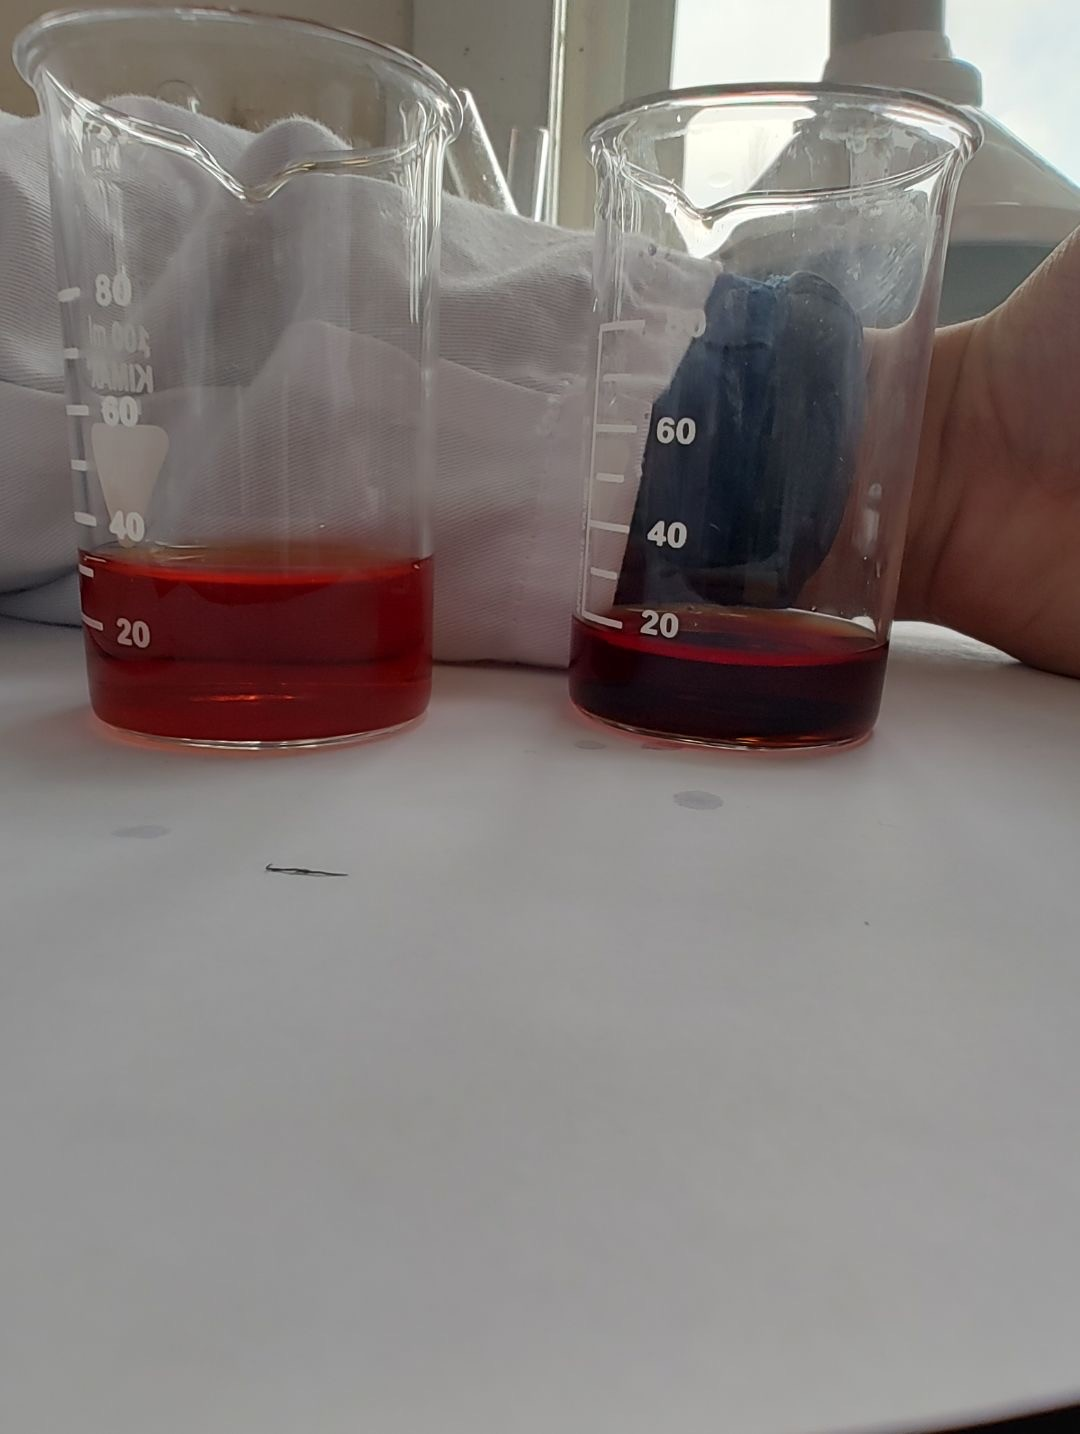
\includegraphics[scale=0.23]{for7b.jpeg}
\end{center}
\caption{De to bægerglas set fra siden}
\label{fig:for7b}
\end{figure}
\section*{Efterbehandling og sammenfatning af resultaterne}
\begin{note}
  Vi har brugt faste stoffer ved tilsætningerne til reagensglassene i stedet for opløsninger af de pågældende stoffer, da opløsninger af dem i høj grad ville ændre på volumenet af blandingen.
\end{note}
\subsection*{Delforsøg 1}
Vi kan forklare forskydningen retning via ligevægtsloven.
Vi ser i ligning \ref{eq:ligevægt}, at reaktionsbrøken bliver mindre end $K_c$ ved tilsætningen af \ce{Fe(NO3)3}.
Reaktionsbrøken bliver da "for lille" og indgrebet efterfølges af en forskydning mod højre.
Det stemmer overens med vores iagttagelser, da mere af den røde ion dannes.
\subsection*{Delforsøg 2a}
Ved opløsning af \ce{Fe(NO3)3} i vand sker reaktionen i ligning \ref{eq:opl}.
\begin{equation}
\label{eq:opl}
\begin{split}
  \ce{Fe(NO3)3(s) -> Fe^3+(aq) + 3NO3-(aq)} 
\end{split}
\end{equation}
\ce{Fe^3+}-ionerne giver en gul farve til opløsningen.
Da ascorbinsyre reducerer disse til \ce{Fe^2+}, så bliver opløsningen farveløs.
\subsection*{Delforsøg 2b}
På tilsvarende måde bliver $[\ce{Fe^3+}]$ mindre ved tilsætningen af ascorbinsyre.
Det gør da reaktionsbrøken "for stor" og der sker en forskydning mod venstre, hvilket stemmer overens med Le Chaterliers princip.
Vores resultater, hvor blandingen bliver farveløs giver altså mening.
\subsection*{Delforsøg 3}
Ved tilsætningen af \ce{KSCN} øges $[\ce{SCN-}]$.
Reaktionsbrøken bliver da "for lille" og indgrebet efterfølges af en forskydning mod højre.
Det stemmer overens med vores iagttagelser med at blandingen bliver mere mørkerød, da mere af den røde ion dannes.
\subsection*{Delforsøg 4a}
Ved opløsningen af \ce{AgNO3} får vi \ce{Ag+} i opløsningen og der er da \ce{SCN-} i \ce{KSCN}-opløsningen.
Et ionreaktionsskema for disse ses i \ref{eq:ion}.
\begin{equation}
\label{eq:ion}
\begin{split}
  \ce{Ag+(aq) + SCN-(aq) -> AgSCN(s)} 
\end{split}
\end{equation}
Den dannede ionforbindelse er tungtopløselig i vand og forårsager det hvide bundfald som er i vores resultater.
\subsection*{Delforsøg 4b}
Reaktionen set i \ref{eq:ion} gør både, at $[\ce{SCN-}]$ bliver mindre og hvidt bundfald dannes.
Det gør da reaktionsbrøken "for stor" og der sker en forskydning mod venstre, hvilket stemmer overens med Le Chaterliers princip.
Vores resultater, hvor blandingen bliver mindre rød giver altså mening.
\subsection*{Delforsøg 5+6}
Tabellen i \cref{tab:for5} giver et overblik over de to delforsøg.
\begin{table}[H]
\centering
\begin{tabular}{l|lll|}
\cline{2-4}
\multirow{}{}{}                               & \multicolumn{3}{l|}{\textbf{Indgreb}}                                                                                                                                                                                                                                             \\ \cline{2-4} 
                                                & \multicolumn{1}{l|}{\textbf{\begin{tabular}[c]{@{}l@{}}Reagensglas 5\\ Opvarming\end{tabular}}} & \multicolumn{1}{l|}{\textbf{\begin{tabular}[c]{@{}l@{}}Reagensglas 6\\ Afkøling\end{tabular}}} & \textbf{\begin{tabular}[c]{@{}l@{}}Reagensglas 7\\ Sammenligning\end{tabular}} \\ \hline
\multicolumn{1}{|l|}{\textbf{Iagttagelse}}      & Orange farve                                                                                    & Mørkerød farve                                                                                 & Rød farve                                                                      \\ \cline{1-1}
\multicolumn{1}{|l|}{\textbf{Forklaring}}       & Forskydning mod venstre                                                                         & Forskydning mod højre                                                                          &                                                                                \\ \cline{1-1}
\multicolumn{1}{|l|}{\textbf{Ændring af $K_c$}} & $K_c$ aftager                                                                                   & $K_c$ vokser                                                                                   &                                                                                \\ \hline
\end{tabular}\caption{Tabel med overblik over de to delforsøg}
\label{tab:for5}
\end{table}
Vi ser, at opvarmningen af blandingen forårsager en forskydning mod venstre, og en afkøling forårsager en forskydning mod højre.
Siden forskydningen må følge Le Chateliers princip, så må reaktionen mellem \ce{Fe^3+} og \ce{SCN-} (reaktionen mod højre) være exoterm.
Da reaktionen mod højre er exoterm, så aftager $K_c$ når temperaturen stiger.
\subsection*{Delforsøg 7a}
Blandingernes farve er den samme set oppefra, da stofmængden af farvestoffet ikke er ændret ved fortyndingen, og arealet, hvorpå vi ser er den samme.
Dog er farven mindre rød i den fortyndede blanding set fra siden, da arealet af væsken vi ser er blevet ændret, hvor stofmængden af farvestoffet ikke er.
Dette giver også meget god mening intuitivt set.
\subsection*{Delforsøg 7b}
Ved fortyndingen til det dobbelte volumen bliver blandingen mindre rød.
Altså sker der en forskydning mod venstre.
Dette kan forklares med ligevægtsloven i \ref{eq:ligevægt}.
$[\ce{FeSCN^2+}], [\ce{Fe^3+}]$ og $[\ce{SCN-}]$ bliver halvt så store.
Da bliver nævneren til $\frac{1}{4}$ af det forrige, hvor tælleren bliver $\frac{1}{2}$ af det forrige.
Reaktionsbrøken er derfor "for stor" og forskydningen må være mod venstre, hvilket stemmer overens med vores resultater.
\section*{Mulige fejlkilder}
Det skal bemærkes, at alle vurderinger af blandingernes farve i forhold til den oprindelige opløsning i den koniske kolbe er foretaget kvalitativt via mennesker.
Altså kan det være svært at vurdere farven, dersom ændringen er meget lille.
\section*{Konklusion}
Vi har undersøgt forskydningen af en kemisk ligevægt, hvor jern(3+)ioner reagerer med thiocyanat og danner en rød kompleks ion, ved forskellige indgreb.
Vi har så kigget på opløsningens farve og på den måde kunne bestemme, om der er sket en forskydning mod højre eller venstre ved det specifikke indgreb.
Vi har til sidst brugt Le Chaterliers princip og ligevægtsloven til at forklare forskydningernes retning.
\end{document}
